\documentclass[a4paper,12pt]{report}
\usepackage[utf8]{inputenc}


\usepackage{tikz}
\usetikzlibrary{calc}
\usepackage{subcaption}

\begin{document}

\thispagestyle{empty}

\begin{figure}[h!]
		\centering
		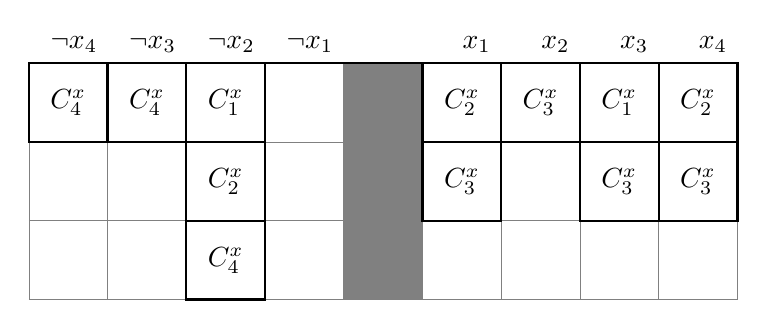
\begin{tikzpicture}
		%grid outline
		\draw[step=1cm,gray,very thin] (-4,0) grid (5,3);
		\fill[gray] (0,0) rectangle (1,3);
		
		%indexes
		\draw[thick] (-4,3) -- (-3,3) node[anchor=south east] {$\lnot x_{4}$};
		\draw[thick] (-3,3) -- (-2,3) node[anchor=south east] {$\lnot x_{3}$};
		\draw[thick] (-2,3) -- (-1,3) node[anchor=south east] {$\lnot x_{2}$};
		\draw[thick] (-1,3) -- (0,3) node[anchor=south east] {$\lnot x_{1}$};
		\draw[thick] (0,3) -- (1,3);
		\draw[thick] (1,3) -- (2,3) node[anchor=south east] {$x_{1}$};
		\draw[thick] (2,3) -- (3,3) node[anchor=south east] {$x_{2}$};
		\draw[thick] (3,3) -- (4,3) node[anchor=south east] {$x_{3}$};
		\draw[thick] (4,3) -- (5,3) node[anchor=south east] {$x_{4}$};
		
		%clauses
		\draw[thick] (-4,3) rectangle (-3,2) node[pos=.5] {$C^x_4$};
		
		\draw[thick] (-3,3) rectangle (-2,2) node[pos=.5] {$C^x_4$};
		
		\draw[thick] (-2,3) rectangle (-1,2) node[pos=.5] {$C^x_1$};
		\draw[thick] (-2,2) rectangle (-1,1) node[pos=.5] {$C^x_2$};
		\draw[thick] (-2,1) rectangle (-1,0) node[pos=.5] {$C^x_4$};
		
		\draw[thick] (1,3) rectangle (2,2) node[pos=.5] {$C^x_2$};
		\draw[thick] (1,2) rectangle (2,1) node[pos=.5] {$C^x_3$};
		
		\draw[thick] (2,3) rectangle (3,2) node[pos=.5] {$C^x_3$};
		
		\draw[thick] (3,3) rectangle (4,2) node[pos=.5] {$C^x_1$};
		\draw[thick] (3,2) rectangle (4,1) node[pos=.5] {$C^x_3$};
		
		\draw[thick] (4,3) rectangle (5,2) node[pos=.5] {$C^x_2$};
		\draw[thick] (4,2) rectangle (5,1) node[pos=.5] {$C^x_3$};
		\end{tikzpicture}
		\caption{The $xorset\_index$ structure.}
		\label{fig:xorset_index}
	\end{figure}

\end{document}
